\section{Specifica Back-End}
  \subsection{SWEDesigner::Server}
    \subsubsection{Informazioni generali}
      \begin{itemize}
        \item \textbf{Descrizione:}\\
        Questo package contiente tutte le componenti del server scritte in JavaScript.
        \item \textbf{Padre: } SWEDesigner
        \item \textbf{Package contenuti:}\\
        \begin{itemize}
          \item Controller \\
          Questo package contiene al suo interno tutti i controller che implementano il pattern MVVM fornito da \glossaryItem{Angular.js}.
          In particolare sono contenuti i Middleware e tutti i Servizi da essi utilizzati.
          \item Model \\
          Questo package contiene tutte le classi utili per la creazione del database, la connessione ad esso e le relative interrogazioni.
        \end{itemize}
      \end{itemize}
    \subsubsection{Classi}
      \paragraph{SWEDesigner::Server::serverLoader}
      	\begin{figure}[h!]
		\centering
		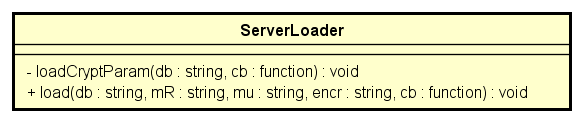
\includegraphics[scale=0.8]{Classi/ServerLoader.png}
		\caption{Diagramma della classe SWEDesigner::Server::serverLoader}
 		\end{figure}
        \begin{itemize}
          \item \textbf{Descrizione:}\\
          Classe che consente il caricamento di tutte le componenti e gli elementi utili al primo avvio dell'applicazione
          \item \textbf{Utilizzo:}\\
          La classe viene utilizzata per il caricamento del server e di tutti i suoi elementi.
          \item \textbf{Metodi:}\\
          \begin{itemize}
            \item \emph{+ load(db: string, mR: string, mu: string, encr: string, cb: function): void}\\
            Si tratta della funzione principale che si occupa di chiamare i metodi load contenuti in tutte le altre classi.
            \item \textbf{Parametri:}\\
            \begin{itemize}
              \item \emph{db: string}\\
              Il path del modulo che gestisce la connessione al database.
              \item \emph{mR: string}\\
              Il path del modulo che gestisce le query.
              \item \emph{mu: string}\\
              Il path del modulo che gestisce il servizio di parsing.
              \item \emph{encr: string}\\
              Il path del modulo che gestisce il servizio di encrypt.
              \item \emph{cb: function}taliano
              Callback che gestisce le rischieste asicnrone al database.
            \end{itemize}
            \item \textbf{- loadCryptParam(db: string, cb: function): void}\\
            Si tratta della funzione utilizzata da load per la richiesta dei parametri crittografici al database.
            \item \textbf{Parametri:}\\
            \begin{itemize}
              \item \emph{db: string}\\
              Il path del modulo che gestisce la connessione al database.
              \item \emph{cb: function}
              Callback che gestisce le rischieste asicnrone al database.
            \end{itemize}
          \end{itemize}
        \end{itemize}
  \subsection{SWEDesigner::Server::Model}
    \subsubsection{Informazioni generali}
      \begin{itemize}
        \item \textbf{Descrizione:}\\
        Questo package contiene tutte le classi e le funzionalità legate al database.
        \item \textbf{Padre: }SWEDesigner::Server
      \end{itemize}
    \subsubsection{Classi}
      \paragraph{SWEDesigner::Server::Model::mongooseConnection}
      	\begin{figure}[h!]
		\centering
		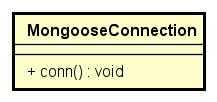
\includegraphics[scale=0.8]{Classi/MongooseConnection.png}
		\caption{Diagramma della classe SWEDesigner::Server::Model::mongooseConnection}
 		\end{figure}
        \begin{itemize}
          \item \textbf{Descrizione: }\\
          Classe che si occupa della connessione al database e degli errori che ne possono derivare
          \item \textbf{Utilizzo: }\\
          La classe viene utilizzata per effettuare la connessione al database all'avvio dell'applicazione.
          \item \textbf{Metodi: }\\
          \begin{itemize}
            \item \emph{+ conn() : void}\\
            Si tratta della funzione che effettua la connessione al database e ne gestisce gli eventuali errori derivanti.
          \end{itemize}
        \end{itemize}
      \paragraph{SWEDesiger::Server::Model::mongooseRequest}
      	\begin{figure}[h!]
		\centering
		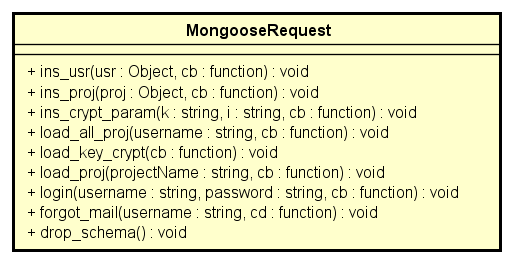
\includegraphics[scale=0.8]{Classi/MongooseRequest.png}
		\caption{Diagramma della classe SWEDesigner::Server::Model::mongooseRequest}
 		\end{figure}
        \begin{itemize}
          \item \textbf{Descrizione: }\\
          Classe che si occupa di gestire tutte le query da e vero il database.
          \item \textbf{Utilizzo: }\\
          La classe viene utilizzata per tutte le richieste, inserimento e fetch, di dati dal e nel database.
          \item \textbf{Metodi: }\\
          \begin{itemize}
            \item \emph{+\texttt{ins\_usr}(usr: Object, cb: function) : void}\\
            Si tratta della funzione che si occupa di inserire un utente all'interno del database.\\
            \item \textbf{Parametri: }\\
            \begin{itemize}
              \item \emph{usr: Object}\\
              L'utente, in formato JSON, da inserire all'interno dello schema.
              \item \emph{cb: function}\\
              Callback che gestisce le richieste asincrone al database.
            \end{itemize}
            \item \emph{+\texttt{ins\_proj}(proj: Object, cb: function) : void}\\
            Si tratta della funzione che si occupa di inserire un progetto all'interno del database.\\
            \item \textbf{Parametri: }\\
            \begin{itemize}
              \item \emph{proj: Object}\\
              Il progetto, in formato JSON, da inserire all'interno dello schema.
              \item \emph{cd: function}\\
              Callback che gestisce le richieste asincrone al database.
            \end{itemize}
            \item \emph{+\texttt{ins\_crypt\_param}(k: string, i: string, cb: function) : void}\\
            Si tratta della funzione che si occupa di inserire una chiave crittografica all'interno del database.\\
            \item \textbf{Parametri: }\\
            \begin{itemize}
              \item \emph{k: string}\\
              La chiave crittografica.
              \item \emph{i: string}\\
              Valore iv per la crittografia.
              \item \emph{cb: function}\\
              Callback che gestisce le richieste asincrone al database.
            \end{itemize}
            \item \emph{+\texttt{load\_all\_proj}(username: string, cb: function) : void}\\
            Si tratta della funzione che si occupa di richiedere tutti i progetti di un dato utente.\\
            \item \textbf{Parametri: }\\
            \begin{itemize}
              \item \emph{username: string}\\
              Nome dell'utente di cui sono richiesti i progetti.
              \item \emph{cd: function}\\
              Callback che gestisce le richieste asincrone al database.
            \end{itemize}
            \item \emph{+\texttt{load\_key\_crypt}(cb: function) : void}\\
            Si tratta della funzione che si occupa di richiedere l'unica chiave crittografica salvata nel database.\\
            \item \textbf{Parametri: }\\
            \begin{itemize}
              \item \emph{cb: function}\\
              Callback che gestisce le richieste asincrone al database.
            \end{itemize}
            \item \emph{+\texttt{load\_proj}(projectName: string, cb: function) : void }\\
            Si tratta della funzione che si occupa di cercare e ritornare un dato progetto.\\
            \item \textbf{Parametri: }\\
            \begin{itemize}
              \item \emph{projectName: string}\\
              Nome del progetto richiesto
              \item \emph{cb: function}\\
              Callback che gestisce le richieste asincrone al database.
            \end{itemize}
            \item \emph{+login(username: string, password: string, cb: function) : void}\\
            Si tratta della funzione che verifica che l'utente che cerca di loggare esiste all'interno del database.\\
            \item \textbf{Parametri: }\\
            \begin{itemize}
              \item \emph{username: string}\\
              L'username dell'utente che cerca di loggare.
              \item \emph{password: string}\\
              La password dell'utente che cerca di loggare.
              \item \emph{cb: function}\\
              Callback che gestisce le richieste asincrone al database.
            \end{itemize}
            \item \emph{+\texttt{forgot\_mail}(username: string, cb: function)}\\
            Si tratta della funzione che restituisce la mail dell'utente dato.\\
            \item \textbf{Parametri: }\\
            \begin{itemize}
              \item \emph{username: string}\\
              Nome dell'utente
              \item \emph{cb: function}\\
              Callback che gestisce le richieste asincrone al database.
            \end{itemize}
            \item \emph{+\texttt{update\_mail}(username: string, mail: string, cb: function)}\\
            Si tratta della funzione che permette di aggiornare il campo mail di un utente.\\
            \item \textbf{Parametri: }
            \begin{itemize}
              \item \emph{username: string}\\
              Nome dell'utente
              \item \emph{mail: string}\\
              Nuova mail
              \item \emph{cb: function}\\
              Callback che gestisce le richieste asincrone al database.
            \end{itemize}
            \item \emph{+\texttt{update\_password}(username: string, password: string, cb: function)}\\
            Si tratta della funzione che permette di aggiornare il campo password di un utente.\\
            \item \textbf{Parametri: }
            \begin{itemize}
              \item \emph{username: string}\\
              Nome dell'utente
              \item \emph{password: string}\\
              Nuova password
              \item \emph{cb: function}\\
              Callback che gestisce le richieste asincrone al database.
            \end{itemize}
            \item \emph{+\texttt{update\_username}(username: string, newUsername: string, cb: function)}\\
            Si tratta della funzione che permette di aggiornare l'username di un utente.\\
            \item \textbf{Parametri: }
            \begin{itemize}
              \item \emph{username: string}\\
              Nome dell'utente
              \item \emph{newUsername: string}\\
              Nuovo username
              \item \emph{cb: function}\\
              Callback che gestisce le richieste asincrone al database.
            \end{itemize}
            \item \emph{+\texttt{update\_proj}(projName: string, usr: string, proj: JSON, cb: function)}\\
            Si tratta della funzione che permette di aggiornare il corpo di un progetto.\\
            \item \textbf{Parametri: }
            \begin{itemize}
              \item \emph{projName: string}\\
              Nome del progetto
              \item \emph{usr: string}\\
              Username dell'utente proprietario del progetto
              \item \emph{proj: JSON}\\
              Corpo del progetto
              \item \emph{cb: function}\\
              Callback che gestisce le richieste asincrone al database.
            \end{itemize}
            \item \emph{+\texttt{update\_nameProj}(projName: string, usr: string, newName: string, cb: function)}\\
            Si tratta della funzione che permette di aggiornare il nome di un progetto.\\
            \item \textbf{Parametri: }
            \begin{itemize}
              \item \emph{projName: string}\\
              Nome del progetto
              \item \emph{usr: string}\\
              Username dell'utente proprietario del progetto
              \item \emph{newName: string}\\
              Nuovo nome del progetto
              \item \emph{cb: function}\\
              Callback che gestisce le richieste asincrone al database.
            \end{itemize}
            \item \emph{+\texttt{login}(mail: string, pwd: string, cb: function)}\\
            Si tratta della funzione che permette di autenticarsi controllando che i dati richiesti dal client esistano nel database.\\
            \item \textbf{Parametri: }
            \begin{itemize}
              \item \emph{mail: string}\\
              E-mail dell'utente.
              \item \emph{pwd: string}\\
              Password dell'utente.
              \item \emph{cb: function}\\
              Callback che gestisce le richieste asincrone al database.
            \end{itemize}
            \item \emph{+\texttt{delete\_user}(username: string, cb: function)}\\
            Si tratta della funzione che elimina un utente dal database.\\
            \item \textbf{Parametri: }
            \begin{itemize}
              \item \emph{username: string}\\
              Username dell'utente.
              \item \emph{cb: function}\\
              Callback che gestisce le richieste asincrone al database.
            \end{itemize}
            \item \emph{+\texttt{delete\_proj}(username: string, projName: string, cb: function)}\\
            Si tratta della funzione che elimina un progetto dal database.\\
            \item \textbf{Parametri: }
            \begin{itemize}
              \item \emph{username: string}\\
              Username dell'utente.
              \item \emph{projName: string}\\
              Nome del progetto.
              \item \emph{cb: function}\\
              Callback che gestisce le richieste asincrone al database.
            \end{itemize}
            \item \emph{+\texttt{drop\_schema}() : void}\\
            Si tratta della funzione che elimina il database.
          \end{itemize}
        \end{itemize}
  \subsection{SWEDesigner::Server::Controller::Middleware}
    \subsubsection{Informazioni generali}
      \begin{itemize}
        \item \textbf{Descrizione: }\\
        In questo package sono definite tutte le componenti middleware del server scritte in JavaScript.
        \item \textbf{Padre: }SWEDesigner::Server::Controller
      \end{itemize}
    \subsubsection{Classi}
      \paragraph{SWEDesigner::Server::Controller::Middleware::midLoader}
      	\begin{figure}[h!]
		\centering
		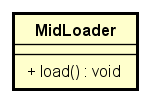
\includegraphics[scale=0.8]{Classi/MidLoader.png}
		\caption{Diagramma della classe SWEDesigner::Server::Controller::Middleware::midLoader}
 		\end{figure}
        \begin{itemize}
          \item \textbf{Descrizione: }\\
          La classe contenente i metodi di caricamento dei servizi utilizzati dalle componenti middleware
          \item \textbf{Utilizzo: }\\
          La classe viene utilizzata all'avvio dell'applicazione per caricare tutto cià che serve per il funzionamento del middleware.
          \item \textbf{Metodi:}\\
          \begin{itemize}
            \item \emph{+load() : void}\\
            La funziona carica il servizio di parsing
          \end{itemize}
        \end{itemize}
      \paragraph{SWEDesigner::Server::Controller::Middleware::Parse}
      	\begin{figure}[h!]
		\centering
		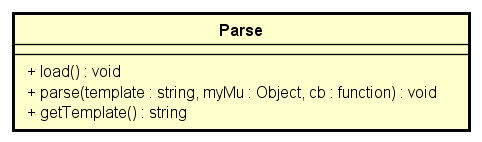
\includegraphics[scale=0.8]{Classi/Parse.png}
		\caption{Diagramma della classe SWEDesigner::Server::Controller::Middleware::Parse}
 		\end{figure}
        \begin{itemize}
          \item \textbf{Descrizione: }\\
          La classe si occupa di gestire il caricamento del template e di richiamare il servizio di parsing
          \item \textbf{Utilizzo: }\\
          La classe viene utilizzata sia per il caricamento del template all'avvio dell'applicazione, sia per richiamare il servizio di parsing quando il client lo richiede.
          \item \textbf{Metodi: }\\
          \begin{itemize}
            \item \emph{+load() : void}\\
            La funzione si occupa di ripulire la cache, compilare il template e caricarlo in cache.
            \item \emph{+parse(template: Object, myMu: Object, cb: function) : void}\\
            La funzione si occupa di richiamare la funzione di parsing del relativo servizio
            \item \textbf{Parametri: }\\
            \begin{itemize}
              \item \emph{template: Object}\\
              Il template precompilato da Moustache.
              \item \emph{myMu: Object}\\
              L'oggetto JSON di cui è necessario il parsing.
              \item \emph{cb: function}\\
              Callback che gestisce la chiamata asincrona al modulo di Moustahce.
            \end{itemize}
            \item \emph{+getTemplate() : string}\\
            La funzione ritorna il percorso in cui è contenuto il template, compilato o meno.
          \end{itemize}
        \end{itemize}
      \paragraph{SWEDesigner::Server::Controller:Middleware::Encrypt}
      	\begin{figure}[h!]
		\centering
		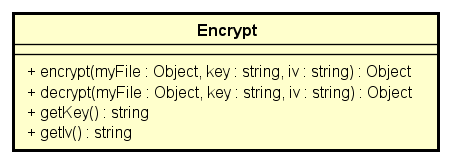
\includegraphics[scale=0.8]{Classi/Encrypt.png}
		\caption{Diagramma della classe SWEDesigner::Server::Controller::Middleware::Encrypt}
 		\end{figure}
        \begin{itemize}
          \item \textbf{Descrizione: }\\
          La classe si occupa di gestire le funzionalità del servizio di encrypt.
          \item \textbf{Utilizzo: }\\
          La classe viene utilizzata per chiamare le funzioni di encrypt del relativo servizio.
          \item \textbf{Metodi:}\\
          \begin{itemize}
            \item \emph{+encrypt(myFile: Object, key: string, iv: string) : Object}\\
            La funzione si occupa di richiamare la funzione di encrypt del relativo servizio e ritorna il file crittato correttamente.
            \item \textbf{Parametri: }\\
            \begin{itemize}
              \item \emph{myFile: Object}\\
              Oggetto JSON da crittare
              \item \emph{key: string}\\
              Chiave crittografica
              \item \emph{iv: string}\\
              IV necessario per la crittografia in AES
            \end{itemize}
            \item \emph{+decrypt(myFile: Object, key: string, iv: string) : Object}\\
            La funzione si occupa di richiamare la funzione di decrypt del relativo servizio e ritorna il JSON decriptato.
            \item \textbf{Parametri: }\\
            \begin{itemize}
              \item \emph{myFile: Object}\\
              Oggetto JSON da crittare
              \item \emph{key: string}\\
              Chiave crittografica
              \item \emph{iv: string}\\
              IV necessario per la crittografia in AES
            \end{itemize}
            \item \emph{+getKey() : void}\\
            La funzione si occupa di richiamare la funzione di generazione della chiave crittografica del relativo servizio.
            \item \emph{+getI() : void}\\
            La funzione si occupa di richiamare la funzione di generazione del valore iv per la crittografia del relativo servizio.
          \end{itemize}
        \end{itemize}
  \subsection{SWEDesigner::Server::Controller::Services}
    \subsubsection{Informazioni generali}
      \begin{itemize}
        \item \textbf{Descrizione: }\\
        Questo package contiene tutti i servizi utilizzati dal middleware del server scritti in JavaScript.
        \item \textbf{Padre: }SWEDesigner::Server::Controller
      \end{itemize}
    \subsubsection{Classi}
      \paragraph{SWEDesigner::Server::Controller::Services::parseService}
      	\begin{figure}[h!]
		\centering
		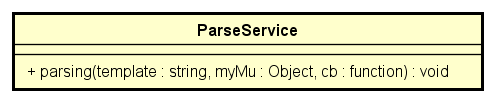
\includegraphics[scale=0.8]{Classi/ParseService.png}
		\caption{Diagramma della classe SWEDesigner::Server::Controller::Services::parseService}
 		\end{figure}
        \begin{itemize}
          \item \textbf{Descrizione:}\\
          La classe si occupa di renderizzare il template pre-compilato e generare, così, un file scritto in Java.
          \item \textbf{Utilizzo:}\\
          La classe viene utilizzata ogni volta che il client richiede la generazione di codice Java a partire dai diagrammi UML disegnati.
          \item \textbf{Metodi:}\\
          \begin{itemize}
            \item \emph{+parsing(template: string, myMu: Object, cb: function) : void}\\
            La funzione renderizza il template pre-compilato in fase di avvio dell'applicazione generando, a fronte dell'oggetto JSON inviato, un file in Java.
            \item \textbf{Parametri: }\\
            \begin{itemize}
              \item \emph{template: string}\\
              Il percorso del template precompilato da Moustache.
              \item \emph{myMu: Object}\\
              L'oggetto JSON di cui è necessario il parsing.
              \item \emph{cb: function}\\
              Callback che gestisce la chiamata asincrona al modulo di Moustahce.
            \end{itemize}
        \end{itemize}
       \end{itemize}
      \paragraph{SWEDesigner::Server::Controller::Services::encryptService}
      	\begin{figure}[h!]
		\centering
		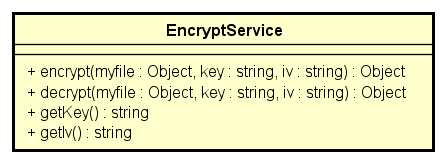
\includegraphics[scale=0.8]{Classi/EncryptService.png}
		\caption{Diagramma della classe SWEDesigner::Server::Controller::Services::encryptService}
 		\end{figure}
        \begin{itemize}
          \item \textbf{Descrizione: }\\
          La classe si occupa di tutti i servizi legati alla crittografia.
          \item \textbf{Utilizzo: }\\
          La classe viene utilizzata per generare le chiavi crittografiche da salvare nel database al primo avvio, qualora queste non esistessero, e di realizzare tutti i servizi legati alla crittografia, quindi encrypt e decrypt.
          \item \textbf{Metodi: }\\
            \begin{itemize}
            \item \emph{+encrypt(myFile: Object, key: string, iv: string) : Object}\\
            La funzione si occupa di criptare il file in arrivo mediante codifica AES utilizzando gli algoritmi di Forge.
            \item \textbf{Parametri: }\\
            \begin{itemize}
              \item \emph{myFile: Object}\\
              Oggetto JSON da crittare
              \item \emph{key: string}\\
              Chiave crittografica
              \item \emph{iv: string}\\
              IV necessario per la crittografia in AES
            \end{itemize}
            \item \emph{+decrypt(myFile: Object, key: string, iv: string) : Object}\\
            La funzione si occupa di decriptare il file in arrivo mediante gi algritmi di Forge.
            \item \textbf{Parametri: }\\
            \begin{itemize}
              \item \emph{myFile: Object}\\
              Oggetto JSON da crittare
              \item \emph{key: string}\\
              Chiave crittografica
              \item \emph{iv: string}\\
              IV necessario per la crittografia in AES
            \end{itemize}
             \item \emph{+getKey() : string}\\
             La funzione genera, tramite Forge, una chiave crittografica e la ritorna.
             \item \emph{+getIv() : string}\\
             La funzione genera, tramite Forge, un gruppo di iv e lo ritorna.
          \end{itemize}
        \end{itemize}
